\subsection{Radian Measure}

\begin{tcolorbox}[title=Problem 2, breakable]
    Give the following values in radians,
    as a fractional multiple of $\pi$.

    (a) $20$\textdegree

    (b) $40$\textdegree

    (c) $140$\textdegree

    (d) $310$\textdegree
\end{tcolorbox}

\textbf{Solution (a):}
\[\frac{20}{360} \cdot 2 \pi\]

\textbf{Solution (b):}
\[\frac{40}{360} \cdot 2 \pi\]

\textbf{Solution (c):}
\[\frac{140}{360} \cdot 2 \pi\]

\textbf{Solution (d):}
\[\frac{310}{360} \cdot 2 \pi\]

\subsection{Sine and Cosine}

\begin{tcolorbox}[title=Problem 3, breakable]
    When the angle $A$ has its defining ray in the fourth quadrant,
    determine whether the sine is positive or negative. Repeat for the cosine.
\end{tcolorbox}

\textbf{Solution:} Sine is negative and cosine is positive.

\begin{tcolorbox}[title=Problem 4, breakable]
    A boat $B$ starts from a point $P$ and moves along 
    a straight river. An observer $O$ stands at a distance 
    of $600$ ft from $P$, on the perpendicular to the 
    river passing through $P$. Find
    the distance from the boat to the observer
    when the angle $\theta$ formed by $B$, $O$,
    and $P$ has 

    (a) $\pi/6$ radians 

    (b) $\pi/4$ radians 

    (c) $\pi/3$ radians
\end{tcolorbox}

\textbf{Solution (a):} $\cos(\pi/6) = \frac{600}{c} \iff c = \frac{600}{\cos(\pi/6)}$ ft

\textbf{Solution (b):} $\cos(\pi/4) = \frac{600}{c} \iff c = \frac{600}{\cos(\pi/4)}$ ft

\textbf{Solution (c):} $\cos(\pi/3) = \frac{600}{c} \iff c = \frac{600}{\cos(\pi/3)}$ ft

\begin{tcolorbox}[title=Problem 5, breakable]
    A balloon $B$ starts from a point $P$
    on earth and goes straight up. A man $M$
    is at a distance of $\frac{1}{2}$ mi from $P$.
    After $2$ min, the angle $\theta$ formed by 
    $P$, $M$, $B$ has a cosine equal to 

    (a) $0.3$

    (b) $0.4$

    (c) $0.2$

    Find the distance between the man and the baloon at that time.
\end{tcolorbox}

\textbf{Solution (a):} $\cos(\theta) = \frac{1/2}{c} = 0.3 \iff c = \frac{1/2}{0.3}$ mi

\textbf{Solution (b):} $\cos(\theta) = \frac{1/2}{c} = 0.4 \iff c = \frac{1/2}{0.4}$ mi

\textbf{Solution (c):} $\cos(\theta) = \frac{1/2}{c} = 0.2 \iff c = \frac{1/2}{0.2}$ mi

\subsection{The Graphs}

\begin{tcolorbox}[title=Problem 2, breakable]
    Sketch the graph of $\sin(2x)$, i.e. all points whose coordinates are $(x, \sin(2x))$.
\end{tcolorbox}

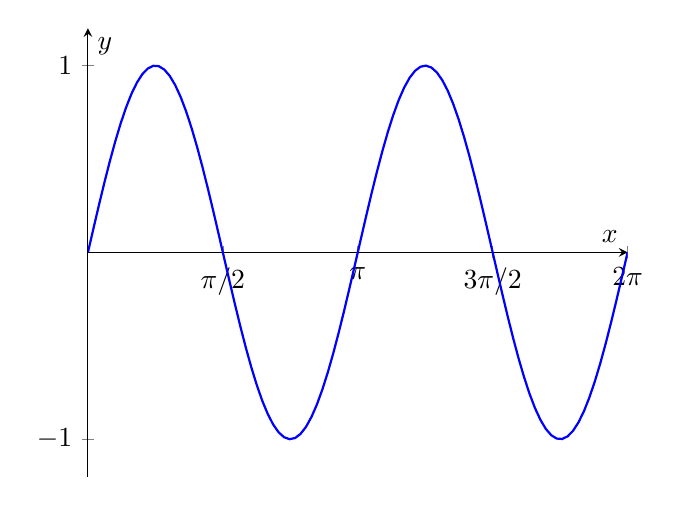
\begin{tikzpicture}
    \begin{axis}[
        axis lines = middle,
        xlabel = $x$,
        ylabel = $y$,
        domain=0:2*pi,
        samples=100,
        ymin=-1.2, ymax=1.2,
        xtick={0,pi/2,pi,3*pi/2,2*pi},
        xticklabels={$0$,$\pi/2$,$\pi$,$3\pi/2$,$2\pi$},
        ytick={-1,0,1}
    ]
        \addplot [blue, thick] {sin(deg(2*x))};
    \end{axis}
\end{tikzpicture}

\subsection{The Tangent}

\begin{tcolorbox}[title=Problem 2, breakable]
    Discuss how the tangent is increasing or decreasing for
    $-\pi/2 < x \le 0$.
    Also for $\pi/2 < x < 3\pi/2$ and $-3\pi/2 < x < -\pi/2$.
\end{tcolorbox}

\textbf{Solution:} Consider $-\pi/2 < x \le 0$.
As $x$ goes from $-\pi/2$ to $0$,
$\sin(x)$ increases and $\cos(x)$ increases.
\begin{center}
\begin{tabular}{c|c|c}
$x$ & $\tan(x)$ \\ \hline
$- \pi/4$ & $-1$ \\
$- \pi/6$ & $-0.577$
\end{tabular}
\end{center}
Thus the ratio $\tan(x) = \frac{\sin(x)}{\cos(x)}$ increases.

Consider $\pi/2 < x < 3\pi/2$.
As $x$ goes from $\pi/2$ to $3\pi/2$,
$\sin(x)$ decreases and $\cos(x)$ decreases.
\begin{center}
\begin{tabular}{c|c|c}
$x$ & $\tan(x)$ \\ \hline
$2\pi/3$ & $-1.732$ \\
$5\pi/6$ & $-0.577$
\end{tabular}
\end{center}
Thus the ratio $\tan(x)=\frac{\sin(x)}{\cos(x)}$ increases.

\begin{tcolorbox}[title=Problem 3, breakable]
    Define the \textbf{cotangent} $\cot(x) = 1/\tan(x)$.
    Draw an approximate graph for hte cotangent, i.e.
    for the points $(x, \cot(x))$.
\end{tcolorbox}

\begin{figure}[h!]
    \centering
    \includegraphics[scale=0.5]{images/inverse_tan.png}
\end{figure}

\begin{tcolorbox}[title=Problem 4, breakable]
    Define the secant and cosecant by 
    \[\sec(x) = \frac{1}{\cos(x)} \text{ and } cosec(x) = \frac{1}{\sin(x)}\]
    for values of $x$ where $\cos(x) \ne 0$ and $\sin(x) \ne 0$, respectively.
    Find enough values of the secant and cosecant until you feel 
    that you have the hang of things. Draw their graphs.
\end{tcolorbox}

\begin{figure}[h!]
    \centering
    \includegraphics[scale=0.5]{images/inverse.png}
\end{figure}

\begin{tcolorbox}[title=Problem 5, breakable]
    Prove that $1 + \tan^2 x = \sec^2 x$.
\end{tcolorbox}

\begin{proof}
    \begin{align*}
        &1 + \tan^2 x = \sec^2 x \\
        \iff &1 + \tan^2 x = \frac{1}{\cos^2 x} \\
        \iff &\cos^2 x + \cos^2 x \tan^2 x = 1 \\
        \iff &\cos^2 x + \cos^2 x \frac{\sin^2 x}{\cos^2 x} = 1 \\
        \iff &\cos^2 x + \sin^2 x = 1 
    \end{align*}
\end{proof}

\begin{tcolorbox}[title=Problem 6, breakable]
    State and prove a similar forumla relating the cotangent and cosecant.
\end{tcolorbox}

\begin{proof}
    \begin{align*}
        &1 + \cot^2 x = \csc^2 x \\
        \iff &1 + \cot^2 x = \frac{1}{\sin^2 x} \\
        \iff &\sin^2 x + \sin^2 x \cot^2 x = 1 \\
        \iff &\sin^2 x + \sin^2 x \frac{\cos^2 x}{\sin^2 x} = 1 \\
        \iff &\sin^2 x + \cos^2 x = 1
    \end{align*}
\end{proof}

\begin{tcolorbox}[title=Problem 9, breakable]
    You are looking at a tall building from a distance of $500$ ft.
    The angle formed by the base of the building, your eyes,
    and the top of the building has 

    (a) $\pi/4$ radians 

    (b) $\pi/3$ radians 

    (c) $\pi/6$ radians 

    Find the height of the buildling.
\end{tcolorbox}

\textbf{Solution (a):} $\tan(\pi/4) = \frac{h}{500} \iff h = 500 \cdot \tan(\pi/4)$ ft

\textbf{Solution (b):} $\tan(\pi/3) = \frac{h}{500} \iff h = 500 \cdot \tan(\pi/3)$ ft

\textbf{Solution (c):} $\tan(\pi/6) = \frac{h}{500} \iff h = 500 \cdot \tan(\pi/6)$ ft

\subsection{Addition Formulas}

\begin{tcolorbox}[title=Problem 1, breakable]
    Find $\sin(7\pi/12)$. [Hint: Write $7\pi/12 = 4\pi/12 + 3\pi/12$]
\end{tcolorbox}

\textbf{Solution:}
\[
\sin(7\pi/12) = \sin(4\pi/12 + 3\pi/12) = \sin(\pi/3)\cos(\pi/4) + \cos(\pi/3)\sin(\pi/4) = \frac{\sqrt{6} + \sqrt{2}}{4}
\]

\begin{tcolorbox}[title=Problem 4, breakable]
    Prove the following formulas. They should be memorizied.

    (a) $\sin 2x = 2 \sin x \cos x$

    (b) $\cos 2x = \cos^2 x - \sin^2 x$

    (c) $\cos^2 x = \frac{1 + \cos 2x}{2}$

    (d) $\sin^2 x = \frac{1 - \cos 2x}{2}$
\end{tcolorbox}

\begin{proof}
    \[
    \sin 2x = \sin(x + x) = \sin x \cos x + \cos x \sin x = \cos x (\sin x + \sin x) = 2 \sin x \cos x
    \]
\end{proof}

\begin{proof}
\[
\cos 2x = \cos(x + x) = \cos x \cos x - \sin x \sin x = \cos^2 x - \sin^2 x
\]
\end{proof}

\begin{proof}
\[
\cos 2x = \cos^2 x - \sin^2 x = \cos^2 x - (1 - \cos^2 x) = 2 \cos^2 x - 1 
\implies \cos^2 x = \frac{1 + \cos 2x}{2}
\]
\end{proof}

\begin{proof}
\[
\cos 2x = \cos^2 x - \sin^2 x = 1 - \sin^2 x - \sin^2 x = 1 - 2 \sin^2 x 
\implies \sin^2 x = \frac{1 - \cos 2x}{2}
\]
\end{proof}

\begin{tcolorbox}[title=Problem 12, breakable]
    (a) A person throws a heavy ball at an angle $\theta$
    from the ground. Let $d$ be the distance from the person to the point where the ball
    strikes the ground.
    Then $d$ is given by 
    \[d = \frac{2v^2}{2} \sin \theta \cos \theta\]
    where $v, g$ are constants. For what value of $\theta$
    is the distance maximum? [Hint: Give another expression for $2 \sin \theta \cos \theta$]

    (b) You are watering the lawn, and point the watering hose at an angle 
    of $\theta$ degrees from the ground. The distance from the nozzle at which the water strikes 
    the ground is giving by 
    \[d = 2 c \sin \theta \cos \theta\]
    where $c$ is a constant. For what value of $\theta$ is the distance 
    at a maximum?
\end{tcolorbox}

\textbf{Solution (a):}
We have \[d = \frac{2v^2}{2}\cos \theta \sin \theta   
            = \frac{v^2}{2}(\sin \theta \cos \theta + \sin \theta \cos \theta)   
            = \frac{v^2}{2}(\sin(2\theta))\]
Now $\sin(2\theta)$ is maximial at $1$ thus we require $\sin(2\theta) = 1$
    and it follows that $\theta = \pi/4$.

\textbf{Solution (b):}
Similar to part (a). 
\[d = c(\sin \theta \cos \theta + \sin \theta \cos \theta)  = c\sin(2\theta)\]
 and it follows that $\theta = \pi/4$.

\begin{tcolorbox}[title=Problem 13, breakable]
    Prove the following formulas for any integer $m, n$:
    \[\sin mx \sin nx = \frac{1}{2}[\cos(m - n)x - \cos(m + n)x]\]
    \[\sin mx \cos nx = \frac{1}{2}[\sin(m + n)x + \sin(m - n)x]\]
    \[\cos mx \cos nx = \frac{1}{2}[\cos(m + n)x + \cos(m - n)x]\]
\end{tcolorbox}

\[
\frac{1}{2}[\cos(m-n)x - \cos(m+n)x] 
= \frac{1}{2}[(\cos mx \cos nx + \sin mx \sin nx) - (\cos mx \cos nx - \sin mx \sin nx)] 
= \sin mx \sin nx
\]

\[
\frac{1}{2}[\sin(m+n)x + \sin(m-n)x] 
= \frac{1}{2}[(\sin mx \cos nx + \cos mx \sin nx) + (\sin mx \cos nx - \cos mx \sin nx)] 
= \sin mx \cos nx
\]

\[
\frac{1}{2}[\cos(m+n)x + \cos(m-n)x] 
= \frac{1}{2}[(\cos mx \cos nx - \sin mx \sin nx) + (\cos mx \cos nx + \sin mx \sin nx)] 
= \cos mx \cos nx
\]

\subsection{Rotations}

\begin{tcolorbox}[title=Problem 2, breakable]
    In the following case, write the matrix 
    associated with the rotation of $G_{\varphi}$,
    when $\varphi$ has the indicated value.
    Write explicitly the coordinates 
    $(x', y')$ of $G_{\varphi}(P)$ if $P$ has 
    coordinates $(x, y)$.

    $\varphi = \pi/4$.
\end{tcolorbox}

\[\begin{bmatrix}
    \cos \pi/4 & -\sin \pi/4 \\
    \sin \pi/4 & \cos \pi/4
\end{bmatrix} \begin{bmatrix}
    x \\
    y
\end{bmatrix} = \begin{bmatrix}
    x' \\
    y'
\end{bmatrix}\]
\[x' = (\cos \pi/4)x - (\sin \pi/4)y, y' = (\sin \pi/4)x + (\cos \pi/4)y\]

\begin{tcolorbox}[title=Problem 21, breakable]
    Associate a matrix with a dilation by $r$.
    Interpret dilation by $r$ in terms of 
    the matrix muliplication.
    Do the same for mixed dilations of type which we have 
    written $F_{a, b}$.
\end{tcolorbox}

\textbf{Dilation:}
\[
\begin{bmatrix}
r & 0 \\
0 & r
\end{bmatrix}.
\]
\textbf{Mixed Dilation:}
\[
\begin{bmatrix}
a & 0 \\
0 & b
\end{bmatrix}.
\]


\begin{tcolorbox}[title=Problem 22, breakable]
    Write down the matrices for the rotations
        $G_{\varphi}, G_{\psi}, G_{\varphi + \psi}$
\end{tcolorbox}

\[\begin{bmatrix}
    \cos \varphi & -\sin \varphi \\
    \sin \varphi & \cos \varphi
\end{bmatrix}\]
\[\begin{bmatrix}
    \cos \psi & -\sin \psi \\
    \sin \psi & \cos \psi
\end{bmatrix}\]
\[\begin{bmatrix}
    \cos \varphi + \psi & -\sin \varphi + \psi \\
    \sin \varphi + \psi & \cos \varphi + \psi
\end{bmatrix}\]